\section{Load Balance}
\label{sec:motivate}

{\em Load balance} is critical to the performance of a distributed storage
system.  We consider two aspects of load balance, namely {\em read balance}
and {\em storage balance}, in which the system reads and stores the same (or
similar) amount of data via each node, respectively.  In storage systems with
homogeneous nodes and without deduplication, storage balance evenly distributes
data across nodes, and hence also implies read balance.  Storage balance can
be achieved by round-robin or random data placements.  When erasure coding is
used, {\em parity declustering} \cite{Holland94} can balance data and parity
distribution by placing stripes across different subsets of nodes (assuming
that the number of nodes is larger than the stripe size $n$). 

In this work, we define the {\em baseline} policy for conventional data
placement as follows. If the number of storage nodes is equal to the erasure 
coding stripe size, then we assign the data chunks to storage nodes in the
round-robin fashion and keep the parity chunks rotated across stripes.
Otherwise, if the number of storage nodes is larger than the erasure coding
stripe size, then we first randomly select the same number of storage nodes as
the stripe size as in parity declustering, followed by assigning the data
chunks to the selected nodes in a round-robin fashion and keeping the parity
chunks rotated across stripes. 

%, which writes chunks across different nodes in a round-robin fashion.  

%\textit{Load balancing} is one of the most significant concerns in designing a data distribution algorithm. 
%By load balancing, it not only indicates balancing the disk consumption on each storage node, but can also imply balancing the amount of data that are targeted at each storage node in a data write.
%The former balancing avoids the case that the capacity of one of the storage nodes is used up before others, and the latter one improves the write throughput by utilizing high write concurrency.
%Existing systems either randomly distribute data to storage nodes favoring nodes with less utilized disks, like that in GPFS \cite{Schmuck02} or distribute data to different storage nodes in a round-robin fashion, like that in FAB \cite{Saito04}, to achieve the load balance.
%
%In current distribution storage systems, several new factors pose challenges to existing load balancing designs.
%First, the introduction of erasure codes requires a storage system to balance not only the data load but also load of the redundancy generated by erasure codes so that potential degraded reads and recovery traffic can be balanced.
%In addition, most distributed storage systems consist of larger number of storage nodes than its coding stripe size, and how to distribute data of a stripe to the large storage pool also deserves thorough design.
%\textit{Parity declustering} \cite{holland92} handles both the data balance and the redundancy balance in such kind of distributed storage systems in a systematic way.

\begin{figure}[!h]
\centering
\subfigure[Files to be written]{
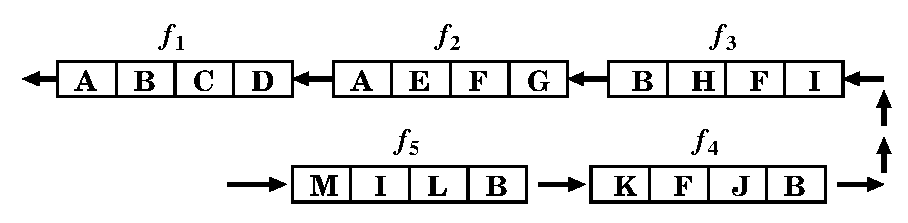
\includegraphics[width=\linewidth]{example.eps}
\label{fig:example_file}
}
\\
\subfigure[Without deduplicateslication]{
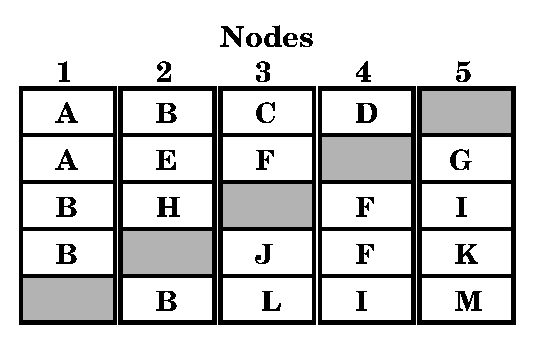
\includegraphics[width=3in]{conv.eps}
\label{fig:example_conv1}
}
\subfigure[With deduplication]{
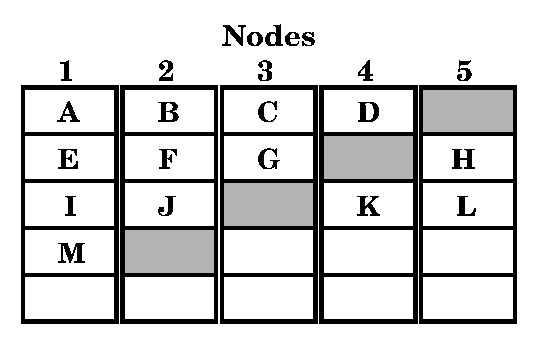
\includegraphics[width=3in]{ddp.eps}
\label{fig:example_conv2}
}
\caption{Layouts of the baseline policy with/without deduplication (the data
and parity chunks are represented in white and gray colors, respectively).}
\label{fig:example}
\end{figure}

\begin{table}[!t]
\caption{File read times of the baseline with/without deduplication.}
\vspace{10pt}
\centering
\label{tab:result_read}
\begin{tabular}{cccccc}
\hline
 &   $f_1$  &  $f_2$     &   $f_3$       &  $f_4$  & $f_5$ \\\hline
 baseline (no dedup) & $\alpha/\beta$ & $\alpha/\beta$ & $\alpha/\beta$ & $\alpha/\beta$ & $\alpha/\beta$    \\\hline
 baseline (dedup)    & $\alpha/\beta$ & $2\alpha/\beta$ & $2\alpha/\beta$ & $3\alpha/\beta$& $2\alpha/\beta$  \\\hline
% impr. without dedup & 0\% & 50\% & 50\% & 66.7\% & 50\% \\\bottomrule
\end{tabular}
\end{table}

% Brief Introduction of baseline design
However, with the baseline placement policy, deduplication inherently leads to
uneven data distribution, thereby breaking the connection between read balance
and storage balance.  We motivate this issue via a toy example shown in
Figure~\ref{fig:example}.  Figure~\ref{fig:example_file} shows a stream of
five files with four chunks each, and we write them to a five-node storage
system using $(5,4)$ erasure coding (i.e., each stripe has four data chunks
and one parity chunk).  We assume parallel I/O accesses, in which read/write
requests are issued to the storage system in parallel.  Let $\alpha$ be the
chunk size, and $\beta$ be the I/O bandwidth of each storage node.  

%With deduplication and erasure coding techniques, existing design first
%deduplicates backup files to reduce storage cost with high backup throughput,
%encodes unique data chunks into code chunks, and, finally, distributes
%code chunks to storage nodes with write and storage balancing.  We
%consider this process as the {\em baseline} design in this paper, and an
%example of uploading five files to a storage cluster consisting of five
%nodes following the baseline design is shown in Figure~\ref{fig:example}. 
Figures~\ref{fig:example_conv1} and \ref{fig:example_conv2} show the data
layouts of the baseline policy without and with deduplication (the latter
stores only unique chunks), respectively.  
%{\color{red} Grey chunks indicate 
%parity chunks for erasure coding. As, most of the time except the case of 
%node failures, reading files involves data chunks of each stripe, 
%distributions of parity chunks will not affect read latency of files.} 
With deduplication, although we
write similar numbers of unique chunks to different nodes (the numbers
differ by at most one), the chunks of a file may be clustered in a
single node, thereby increasing the file read time.  For example, three of
four chunks of file~$f_4$ are stored in node~2 (see
Figure~\ref{fig:example_conv2}).  Table~\ref{tab:result_read} shows the
resulting read times of different files.  We observe that the read times of
files $f_2$, $f_3$, $f_4$, and $f_5$ all increase when deduplication is used,
for example, by 2$\times$ or 3$\times$ when compared to without deduplication.
Thus, maintaining storage balance cannot achieve read balance when
deduplication is used. 

The above example only considers homogeneous nodes.  If a storage system
comprises heterogeneous nodes, the file read time distribution can be more
diverse since the chunks of a file may be aggregated in a bottlenecked
node.  Although the above example is contrived, we show via trace-driven
analysis that read imbalance can occur when we apply deduplication to
real-world workloads (see Section~\ref{sec:evaluation}). 

%Illustrative example showing the imbalance in baseline design
%In the baseline design, the number of chunks in the storage system is much smaller than that of a storage system without deduplication.
%For instance, if we want to retrieve file 3 from both of the two systems in
%Figure~\ref{fig:example_conv1} and Figure~\ref{fig:example_conv2}, the
%baseline design is bottlenecked by the three chunks on Node 1 while, in the
%system without deduplication, we only need one concurrent full stripe read to
%download all the required data.  Suppose the chunk size is $\alpha$ (in the
%unit of MB), the I/O capacity of each storage node is $\beta$ (in the
%unit of MB/s) and data chunks of a file can be accessed in
%parallel from each storage node. 

%\textbf{Trace-driven analysis on imbalance on read performance}
%\begin{itemize}
%\item \emph{Trace description}
%\item \emph{Methodology}
%\item \emph{Observation \& Implications}
%\end{itemize}


%We take the daily snapshots of 9 students covering 6 months in the year 2013 as our working dataset. 
%We feed the snapshots of the 9 students to our simulator day by day.
%Each snapshot contains sufficient metadata of chunks of all the files of one student's home directory
%Our simulator simulates the baseline design, and parses each snapshot into stream of metadata of chunks for each file, performs deduplication and erasure codes with the parsed metadata and, finally, records the decision on how code chunks of each file are distributed.
%For each file, we take the largest number of data chunks that we need to download from a storage node as the indicator of read latency of the file.
%And we consider the case where a file can be downloaded by downloading equal number of data chunks from each of the storage nodes in parallel as the optimal case for the file.
%\textbf{(Is it necessary to present profile of the trace? Say, distribution of file size and deduplication ratio here? by Min)}
%For each file, we compare its indicator of read latency under baseline design and that in optimal case, and calculate the ratio of the gap between the indicator under baseline design and that in the optimal case over the indicator under the baseline design.
%The comparison result is shown in Figure~\ref{fig:fsl}. 

%We further simulate the problem using a public trace, called \textit{FSLHOME}
%\cite{tarasov12}, that is published by the File system and Storage Lab (FSL)
%at Stony Brook University.  We observe that, under baseline distribution
%design, the average read balance of all the files in the trace can be
%improved by 24.29\%.  In addition, for around 35\% of the files, it's
%possible to improve the read performance in the baseline design by
%reducing the maximum number of data chunks to be downloaded from a
%storage node by more than 40\%.  We consider this trace as representative
%of user data backup scenario, and, based on our trace study, we believe
%that imbalance of data placement caused by deduplication can drastically
%affect the file read performance in real-world backup storage systems.
%We will talk more about simulation on the FSLHOME trace in
%Section~\ref{sec:evaluation}.


%In addition, we observe that, for around 35\% of files, the gap between the baseline design and the optimal case is more than 40\%. 
%This indicates that, for these files, it's possible to improve the read performance in the baseline design by reducing the maximum number of data chunks to be downloaded from a storage node by more than 40\%.
%Read latency of some files can even be improved by up to 80\%.
%\begin{figure}[!t]

%\centering
%\includegraphics[width=3.2in]{fsl_gap_histo.eps}
%\caption{Histogram of Potential Improvement Ratio from Baseline to Optimal Placement.}
%\label{fig:fsl}
%\end{figure}


%According to the illustrative example, we realize that there exist trade-offs between storage efficiency and data read concurrency in the baseline storage system design. In this work, our main goal is to improve the data access concurrency with lossless storage efficiency same as baseline deduplication storage system. Our main idea is to smartly distribute unique data blocks to nodes according to information, which can be derived by deduplication module, on duplicate blocks. Thus, our data distribution algorithm is \textit{deduplication-aware}. We will show that, in a real distributed storage cluster with other requirements, it is computationally expensive to find the optimal distribution solution by testing all possible distribution strategies. And we will present, \textit{even data placement (EDP)}, a polynomial time algorithm to place unique data so that future reads on each node for a file will be as even as possible. We also extend the distribution problem with cost coefficients to tackle heterogeneity in real storage clusters. Typical heterogeneous cost associated with each storage node includes expense per block of data, download time per block of data, loss probability per block of data and etc. As our work aims at improving file download performance, we take heterogeneity in link bandwidth of each node into consideration, and derive the \textit{cost-based even data placement (CEDP)} algorithm. We show that CEDP can further improve file read performance over EDP in real storage cluster. %\textbf{Min: Introduce heterogeneity as contribution as well [DONE]}

%As storage efficiency is a key dimension in current storage systems, many products, such as Data Domain \cite{zhu08}, HYDRAstor \cite{dubnicki09} and HP \cite{lillibridge09}, incorporate deduplication by default. Therefore, it is urgent to tackle the problem of file level data imbalance induced by data deduplication to improve read performance in reliable deduplication storage clusters.

%\textbf{Problem description}

%We summarize our main contributions as follows:
%\begin{itemize}
%\item \textbf{Problem Introduction} As far as we know, this is the first work that proposes the imbalance problem induced by deduplication in distributed storage systems. We illustrate the problem via illustrative examples. With extensive simulation on real-world datasets, we show that the imbalance problem does exist in real storage clusters.  

%\item \textbf{Problem Investigation} We formulate an optimization problem that maximizes the evenness of data distribution for each file in a distribution storage system with deduplication. We showed that, despite of the complexity from its integral programming nature, the single file distribution problem can be handled by greedy algorithm efficiently. We further enhance the optimization problem via adding extra practical constraints. The first practical constraint is that each node should receive equal number of unique blocks in each batch distribution. To ensure this constraint, we buffer multiple files inside a distribution buffer before optimizing the distribution strategy for all the files. We also extend the problem to adapt to the scenario where nodes have heterogeneous hardware settings, and this will improve the performance of our distribution algorithm in real storage clusters.

%\item \textbf{Even Data Placement Algorithms} We present efficient, polynomial time data placement algorithms to handle the complicated distribution problems online. The algorithm can evenly distribute data blocks based on two types of metrics, either number of blocks of a file on each node or total download time of blocks of a file on each node. We also conduct extensive simulations to validate the efficiency of the algorithms. And the result shows that our data placement algorithm can achieve nearly-optimal distribution of data in most scenarios. %\textbf{Min: Avoid specific name, like BEDP and CEDP, here [DONE]}

%\item \textbf{Implementation and Evaluations} We implement a prototype and evaluate it atop a cluster with XX storage nodes to demonstrate the practicality of the even data placement algorithms.
%\end{itemize}

%The rest of the paper is organized as follows: In Section~\ref{sec:background}, we will introduce several key techniques that are involved in modern distributed storage systems. In Section \ref{sec:formulation}, we formulate the distribution problem as an integer programming problem. We further extend the problem to tackle common constraints in distributed storage systems, including disk load balance and heterogeneity. In Section \ref{sec:algorithm}, we present the even data placement algorithms. In Section \ref{sec:evaluation}, we show evaluations on performance of the even data placement algorithms via simulations.%and experiments on our proto-type.
 
